\chapter{Asset Handling and Basic Game Mechanics}

Graphics and Sounds are the essence of every good game. In the first chapter
you have learned the very basics of \SB{} and \cocos{} by building a game that only
uses plain colored shapes. In this chapter you will learn how \SB{} helps you to
integrate assets into your game. Learning by example is the most fun, so
starting in this chapter and lasting until the end of the book, we will build
a full iOS game! The final product is available on the App Store!%TODO: Add link

Here's what the final game will look like:
\begin{figure}[H]
    \centering
    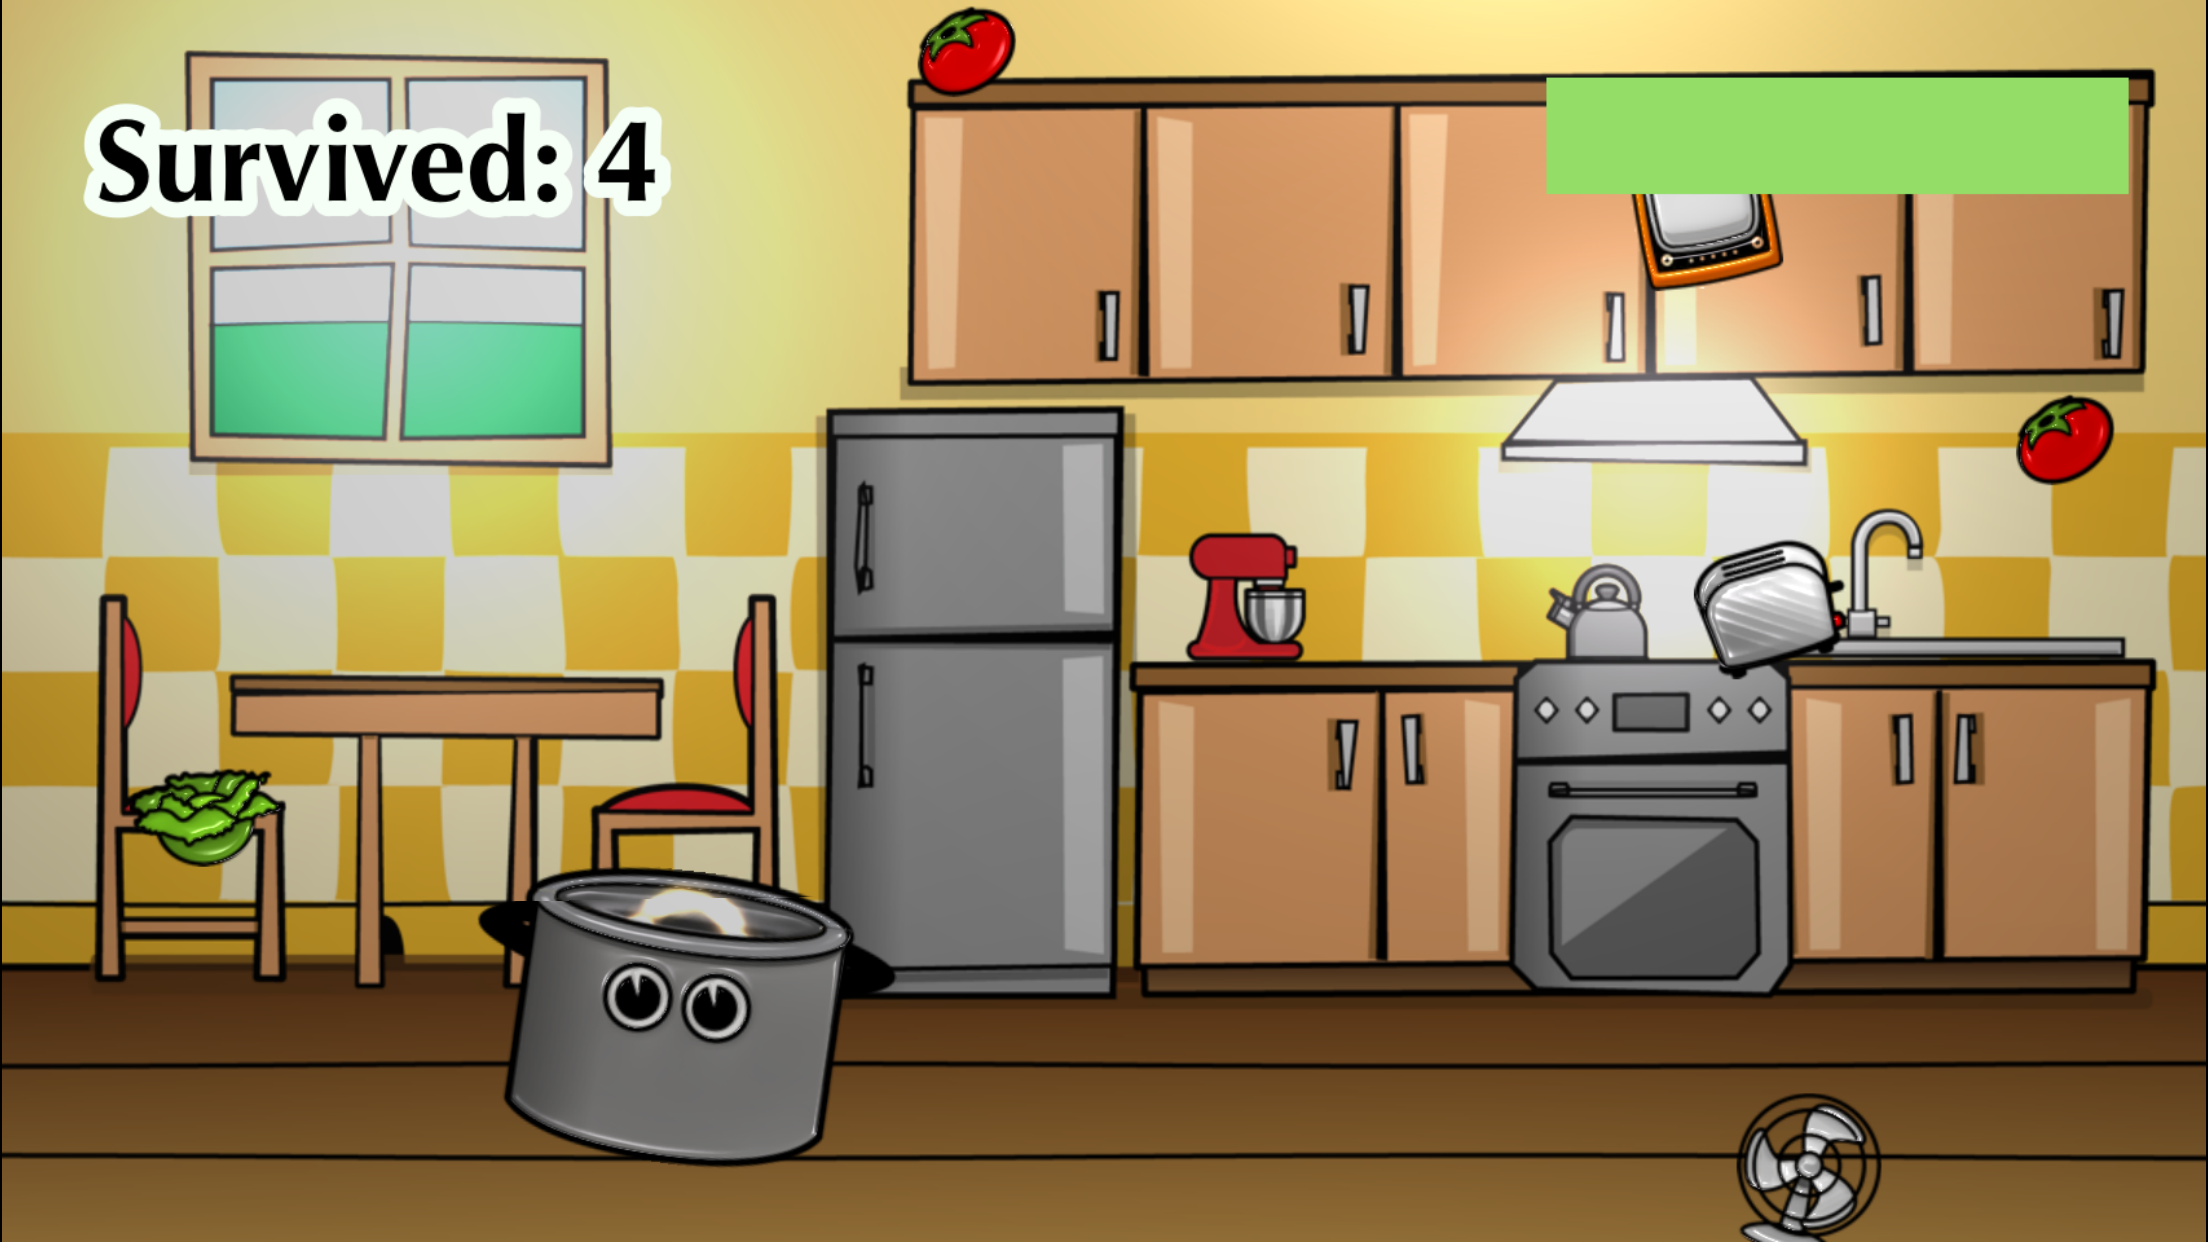
\includegraphics[width=250pt]{images/Chapter2/final_game.png}
    \caption{The game that is built throughout this book}
\end{figure}

The goal of that game is for the user to drag a pot across the screen in order
to collect food items and avoid inedible kitchen equipment and other electronic
devices.

When building this type of game you can choose whether or not to use the
\cocos{} physics engine. For this book I have chosen to build the game
\textbf{without} it. Here are the reasons:
\begin{enumerate}
  \item Games built with a physics engine have a very different feel from games
  where all objects are moved through custom code. A physics engine is never
  100\% accurate. The player can feel this in collisions and other interactions
  throughout the game. This is one of the main reasons while many platformers do
  not rely on physics engines. They are great for game concepts that entirely
  rely on a physics engine - such as the popular game angry birds. But there are
  more games out there that don't use a physics engine than the other way
  round.
  \item Many games are a little bit easier to build with a physics engine, but
  you will end up learning a very different set of skills. The main goal of this
  book is to teach you skills that you can use to build your own games. I felt I
  can provide more value by implementing object movement, collision detection,
  etc. customly.
  \item There are already great resources on physics based games with \SB{} and
  \cocos{} out there, including our Peeved Penguins tutorial
  (\url{https://www.makeschool.com/tutorials/getting-started-with-spritebuilder/}) and 
  Steffen Itterheim's book \textit{Learn SpriteBuilder}
  (\url{http://www.apress.com/9781484202630}).
\end{enumerate}

Now you should have a decent idea of the game we will be building throughout the
rest of this book! Let's get started with the first part: asset
management and setting up the basic mechanics of our game.

\section{Adding Assets to a SpriteBuilder project}
First of all we need to create a new \SB{} project. You will also need to
download the art pack for this game.

\begin{leftbar}
\begin{enumerate}
  \item Create a new \SB{} project and name it \textit{FallingObjects}.
  \item Download the assets from
  \url{https://dl.dropboxusercontent.com/u/13528538/SpriteBuilderBook/assets.zip}.
  \item Unzip the folder once the download completes
  \item Add the assets to the project by dragging the
entire folder into the left \textit{File View} in the left panel of
\SB{}:\index{Assets!Adding Assets}
\begin{figure}[H]
    \centering
    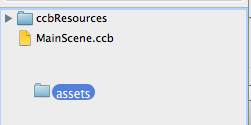
\includegraphics[width=200pt]{images/Chapter2/DragAssets.png}
\end{figure}
\end{enumerate}
\end{leftbar}

Great, now we have some assets to use in our game. Now is a good time to take a
close look at how \SB{} and \cocos{} handle assets.

\section{Asset Handling in \SB{} and \cocos{}}
One of the main goals of \SB{} is to make game development for multiple device
types as easy as possible. This means that games should automatically be able to
run on differently sized iPhones and on iPads. Since each of these
devices has a different resolution \cocos{} and \SB{} allow developers to use different assets to target them. \SB{}
provides four different resolution categories:
\begin{description}
\item[phone] resolution for non-retina iPhone
\item[phone-hd] retina resolution for iPhone
\item[tablet] resolution for non-retina iPad
\item[tablet-hd] resolution for retina iPad
\end{description}

Luckily using \SB{} there is no need to provide four resolutions for each asset
thanks to \textbf{automatic downscaling}\index{Assets!Automatic Downscaling}.
Per default \SB{} assumes that all assets added to a project are provided in \textit{tablet-hd} resolution, then
\SB{} generates downscaled images for the other resolutions. While you can
provide different images for the four targets, \SB{} only knows three resolution
types:
\begin{description}
\item[1x] non-retina images
\item[2x] retina images
\item[4x] double sized retina images
\end{description}

By default \SB{} maps these resolution types to the different devices in a way
that every asset has the same relative size, in relation to the screen size, on
every device. This means games running on an iPad will look very similar to games
running on an iPhone, except that they have a slightly different aspect ratio.
Here is an example from on of our tutorials showing what a game looks like on
different device types:

\begin{figure}[H]
		\centering
		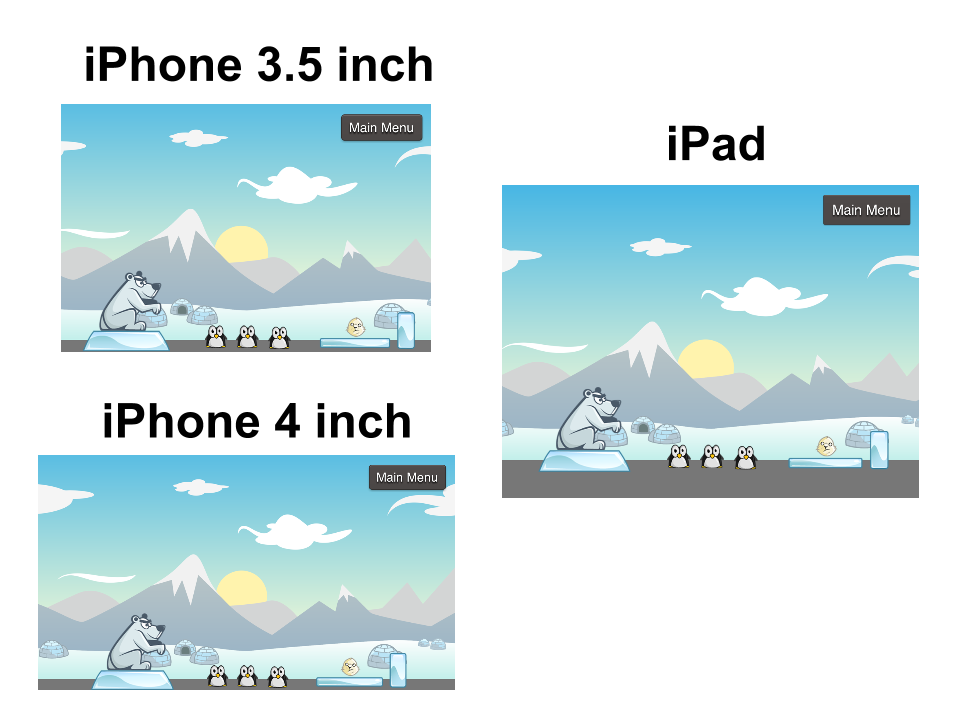
\includegraphics[width=0.9\linewidth]{images/Chapter2/ResultsFlexibleScaleMode.png}
		\caption{From our tutorial \textit{Dynamic Layouts with SpriteBuilder and
		Cocos2D}}
\end{figure}

Let's take a look at all of the options for image sizes in the context of our
\SB{} project - that will make it easier to understand how the parts fit
together.

Let's start in the project settings. When you open the project settings
(\textit{File -> Project Settings\ldots}) you can see the available downscaling options:

\begin{figure}[H]
		\centering
		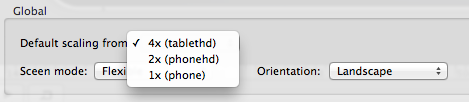
\includegraphics[width=300pt]{images/Chapter2/DownScalingGlobal.png}
\end{figure}

The \textit{Default scaling from} setting defines the \textit{global}
downscaling option, i.e. which resolution \SB{} uses to generate all of our
assets. Individual assets can define their own behaviour, thereby overriding
this global setting. To make support of multiple devices as easy as possible you should provide all of your assets in \textit{4x} resolution and keep this default setting.

When you select an individual asset from the File View you can see different
downscaling settings:

\begin{figure}[H]
		\centering
		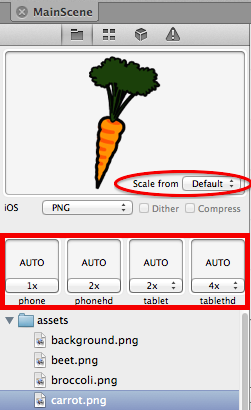
\includegraphics[height=200pt]{images/Chapter2/DownScalingPerAsset.png}
\end{figure}

Each asset can have its own \textit{Scale from} setting. \textit{Default} means
that the global project setting applies (in this project: downscaling from
\textit{4x}). Additionally you can see how the different resolution types are
mapped to the different device types. Here you could for example choose that a
certain asset should not be scaled up on retina tablets by choosing a
\textit{2x} resolution for \textit{tablethd} - however, the default settings
work best most of the time.

For future reference, this is an example that shows you which sizes your assets
will have on the different devices by default:

\begin{table}[H]
\begin{tabular}{llll}
\textbf{Device} & \textbf{Default Resolution Type} & \textbf{Size on Screen (points)} & \textbf{Size in Pixels} \\
iPhone          & 1x                               & 50x50                            & 50x50                   \\
iPhone Retina   & 2x                               & 50x50                            & 100x100                 \\
iPad            & 2x                               & 100x100                          & 100x100                 \\
iPad Retina     & 4x                               & 100x100                          & 200x200                
\end{tabular}
\end{table}

The key takeaway for now is that it's best to provide assets in \textit{4x}
resolution in order to build games that look good on all device types. All the
assets in the art pack that you downloaded earlier are provided in \textit{4x}
resolution.

That's enough of theory for now - let's get started on building the
\textit{Falling Object!} game.

\begin{details}[Different images for different devices] 
You can not only change the scaling option for an asset on different devices,
you can even use an entirely different image for a certain resolution. You can
do that by dragging an image \textbf{that is currently not part of the \SB{}
project} from Finder into one of the four boxes below the asset preview:
\begin{figure}[H]
		\centering
		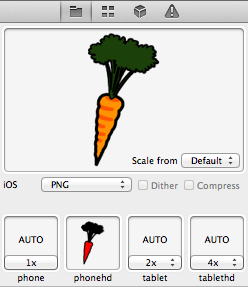
\includegraphics[height=140pt]{images/Chapter2/DifferentImageDevice.png}
\end{figure}

Note that images you add this way will be displayed in exactly the size you have
added them and will not be downscaled.

\end{details}

\begin{details}[Behind the scenes] 
If you are interested in how \SB{} and \cocos{} organize assets you can take a
look at the resource package
(\textit{/Packages/\allowbreak{}SpriteBuilder Resources\allowbreak{}.sbpack}) by
right-clicking and selecting \textit{Show Package Contents}:
\begin{figure}[H]
		\centering
		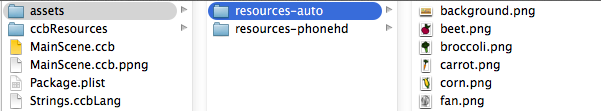
\includegraphics[width=280pt]{images/Chapter2/behindscenes_resourcepack.png}
\end{figure}
You will see that \SB{} groups images inside the assets folder into a
\textit{resources-auto} folder, all images in that folder are subject to
automatic downscaling. If you explicitly add images for a certain resolution as
shown with the carrot in the above example, a new folder for that resolution
(e.g. \textit{resources-phonehd}) is created.

In \cocos{} a class called \inlinecode{CCFileUtils} is responsible for loading
the correct images for the current device during runtime. \SB{} uses a special
configuration of \inlinecode{CCFileUtils} that is set up in
\inlinecode{[CCBReader configureCCFileUtils]}. \index{Framework
Classes!CCFileUtils}
\end{details}

\section{Adding the background image}
Now that we have a basic understanding of how asset management works, lets get
started working on our game. For now it will only consist of one scene, so
we can start working directly in the \textit{MainScene.ccb} that is part of the
\SB{} template. 

\begin{leftbar}
\begin{enumerate}
  \item Open \filemention{MainScene.ccb} in your \SB{} project
  \item Remove all of the content from \filemention{MainScene.ccb} by selecting
  all nodes on stage and hitting the return key
  \item Drag the \filemention{background.png} file from the asset folder, in the
  left panel of \SB{}, to the stage. \SB{} will automatically generate a Sprite
  Node from this image
\end{enumerate}
First, remove the existing content so that we can start with a blank
scene. Now we can add the background image. To add a sprite to a scene we can
simply drag the asset from the left panel to the stage, \SB{} will
automatically create an instance of \ccsprite{}. Add the \textit{background.png} image to the stage.
\end{leftbar}

How should we position this background image? We already have briefly discussed
the \SB{} positioning system (\ref{PositioningSystem}). Using the positioning
system correctly is especially important when we create games that shall work on
both phones and tablets - which we always should try to do. In most cases - like
in this game - it is best to center the background image. That way phones
and tablets will display a very similar portion of it. The background image that
is part of the asset catalog has a size of \textit{(2272 x 1536)}. This is an
image in \textit{4x} resolution that has exactly the right dimensions to support
phones and tablets in landscape mode. It's high enough for the higher tablet
screens and wide enough for the wider phone screens.

Let's position the background image correctly!
\begin{leftbar}
Center the image by choosing a \textit{normalized} position type (\textit{in \%
of parent container}) and setting the position to (50, 50) as shown below:
\begin{figure}[H]
    \centering
    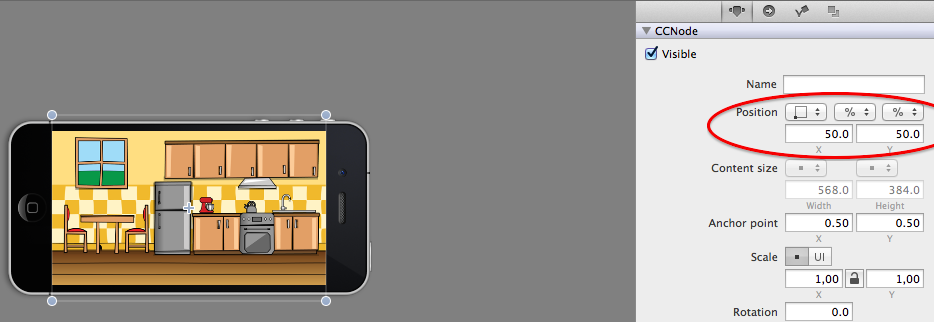
\includegraphics[width=0.9\linewidth]{images/Chapter2/center_background.png}
\end{figure}
\end{leftbar}

You can preview what your game will look like on different device types directly
in \SB{}, without the need to compile and run the game - you should do this as
often as possible! The option is available from the menu \textit{Document ->
Resolution}. You can also use the CMD+1, CMD+2 and CMD+3 shortcuts. This feature
will allow you to preview the game on a 3.5-inch iPhone, a 4-inch iPhone and an
iPad. \label{preview_screen_sizes}

\section{Create falling objects}
Now let's dive into the implementation of the actual game. The next step should
be adding falling objects. Our game will have two categories of objects, ones
that should be caught (food) and ones that shouldn't (electronic devices).

In total we have over ten different objects in our game but these just exist as
visual enhancement, actually we are only differing between two types of objects.
One way to implement the falling objects would be creating a \ccbfile{} for each
object but that isn't actually necessary for this game. We need to create all
falling objects dynamically, while the game is running, and for each object we
only need to store if it should be caught or not. That can be best accomplished
by a subclass of \ccsprite{} that we create in code. This way you will also
learn how to use assets you added in \SB{} to create \ccsprite{}s in code.
\begin{leftbar}
Open the \xcode{} project of the game to get started. Remember that you can use
the \textit{CMD + Shift + O} shortcut to do so!
\end{leftbar}

\subsection{Create a falling object class}
In general we have two ways to differentiate objects a player should catch and
ones he shouldn't catch. We could:
\begin{itemize}
  \item Create two distinct subclasses of \ccsprite{}, each representing one
  type of object
  \item Only have one subclass and add a \inlinecode{type} property to it
\end{itemize}
Since our falling objects won't have any type-specific behaviour, creating two
distinct subclasses is not necessary in this case. Instead, as of now, one
subclass with a \inlinecode{type} property is the better solution.

\begin{leftbar}
Create a new class called \inlinecode{FallingObject} and make it a subclass
of \ccsprite{}. If you run into issues, check how we created new classes in the
last chapter.
\end{leftbar}

The best way to implement our \inlinecode{type} property is using an 
enumeration. Enumerations define multiple mutually exclusive values.

\begin{leftbar}
Add this enum definition to \textit{FallingObject.swift},
inside of the \inlinecode{class} block:

\begin{lstlisting}
enum FallingObjectType: Int {
  case Good
  case Bad
}
\end{lstlisting}
\end{leftbar}
The enumeration above can only be in one of the two states at a time, either
\inlinecode{.Good} or \inlinecode{.Bad}. Swift supports multiple types of
enumerations and enumeration values.
In the example above we are creating an enumeration with \textit{Raw Values}.
When we use an enumeration with raw values we need to assign a type as part of
the enum definition, as shown in the first line (\inlinecode{enum
FallingObjectType: Int}). 

Each enum value will be mapped to one value of this
provided type. In the example shown above, the raw value for
\inlinecode{FallingObjectType.Good} will be 0 and the value for
\inlinecode{FallingObjectType.Bad} will be 1. Thanks to auto-increment we do not
need to map entries to numbers explicitly. Associating enum values with raw values is optional,
throughout this chapter you will see why this feature is useful to us.

\begin{details}[Enumerations in Swift] 
You can read everything about the different ways of creating enumerations in
Swift in the official documentation
(\url{https://developer.apple.com/library/ios/documentation/
Swift/Conceptual/Swift_Programming_Language/Enumerations.html}).
You can also read a more practical tutorial on Swift enums on our website:
(\url{https://www.makeschool.com/tutorials/learn-swift-by-example-part-2-enums})
\end{details}

Additionally we add a property to store the object type. Later we will
add an initializer to set the type of the falling object upon initialization. 

\begin{leftbar}
Add a property to store the falling object type, so that the class looks as
following:
\begin{lstlisting}
import Foundation

class FallingObject: CCSprite {

  enum FallingObjectType: Int {
  case Good
  case Bad
  }
    
  private(set) var type:FallingObjectType
  
}
\end{lstlisting}
\end{leftbar}

We define the property to be \textit{readonly} because we will not
support changing the type of a falling object after it has been created. In Swift we can 
define variables as \textit{readonly} by marking the \textit{setter} as private.

Note that the code will not compile at this point. Since \inlinecode{type} isn't
declared as an optional value, Swift requires us to provide an initializer that
sets this value. We will fix this in the next section.

\subsection{Choosing an asset for a falling object}
We want the game to spawn entirely random falling objects. As you remember we
have a couple of assets for both types of objects. Whenever we spawn an object
we will need to choose a random asset, based on the object type. A good place to
implement this functionality is directly in the \inlinecode{FallingObject}
class. We can provide a custom initializer that allows the class to be initalized with an object type.
When this initializer gets called we choose a random asset and apply it as a
texture to the \inlinecode{FallingObject}.

How can we create a list of images for objects that should be caught (e.g.
food) and ones that shouldn't (e.g. radios)? One way of implementing this would
be creating two arrays, one for each object type, and storing filenames for 
different assets in these arrays. As good game developers however, we try to
keep game content and code as strictly separated as possible. That makes it
easier to update the list of assets later on and it keeps our codebase small and well
structured. So instead of creating these arrays in code we could use some sort
of resources file that stores information on available images. A very common 
format for storing such type of information in iOS applications is a
\textit{plist} (Property List). A plist is a special type of XML file that allows us to
store structured data. The iOS frameworks have some
features that make it easy to interact with plists and to generate them or read
them from source code.

Let's a plist file to our project!

\begin{leftbar}
Create a \textit{plist} by selecting \textit{File ->
New -> File\ldots} from \xcode{}'s menu. 
Then select \textit{Resource} from the left panel and choose
\textit{Property List} on the right:

\begin{figure}[H]
    \centering
    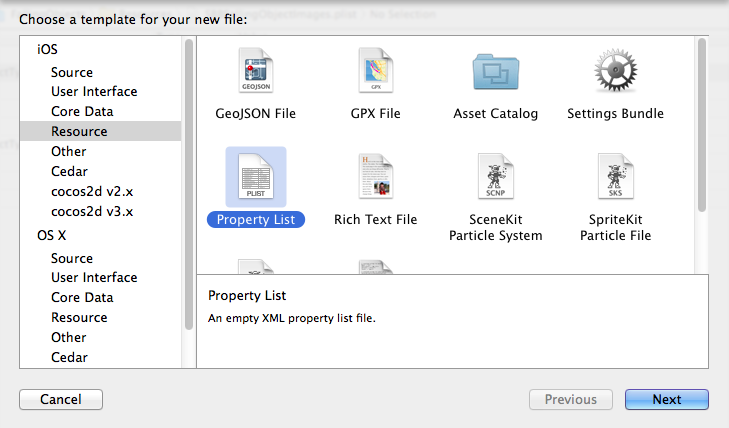
\includegraphics[width=300pt]{images/Chapter2/create_plist.png}
\end{figure}

As the name choose \textit{FallingObjectImages}.
\end{leftbar} 

Next, let's fill the \textit{plist} with two arrays that contain the filenames
of the assets that we added in \SB{}, grouped into \textit{good} and
\textit{bad} objects. 

When referencing assets from a \SB{} project you always
need to include the folder names in which the images are contained. Instead of
referencing the tomato with \inlinecode{tomato.png} you need to use
\inlinecode{assets/tomato.png} since the image is in the \inlinecode{assets}
folder in the \SB{} project.

\begin{leftbar}
\begin{enumerate}
  \item Right-click onto the \textit{plist} root and select \textit{Add Row}
  from the context menu
  \item Click onto the \textit{Type} column of the new row and select the type
  to be \textit{Array}
  \item Double-click onto to the name of the array and rename it to
  \textit{FallingObjectTypeBadImages}
  \item Repeat step 2 and 3 to create another array
  \item Name that new array \textit{FallingObjectTypeGoodImages}
  \item Add all the assets as \textit{String} entries to the according arrays
\end{enumerate}
The resulting \textit{plist} should look like this:
\begin{figure}[H]
    \centering
    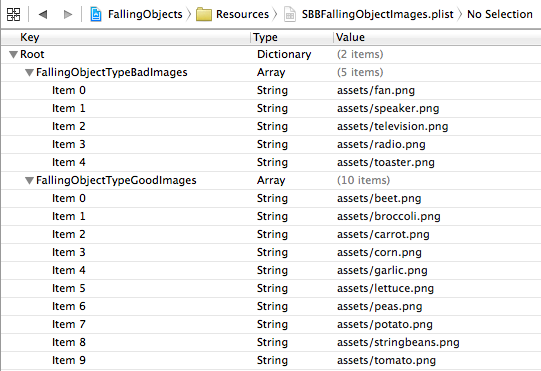
\includegraphics[width=0.7\linewidth]{images/Chapter2/plist_setup.png}
\end{figure}
\end{leftbar}

Now we have a list of all asset names grouped into the two object type
categories. Time to implement the \inlinecode{FallingObject} class.

When a falling object is initialized we want to
choose random image from the \textit{plist} that we just created.
The first step is loading the \textit{plist} in code. Luckily \textit{plists}
consist of Dictionaries, Arrays, Strings, etc. and all of these types exist in
Swift as well - there are some very convenient methods to load
\textit{plists} and turn their content into Swift types. 

During each playing session we are going to create hundreds of
falling objects. Since the images that represent these objects won't change it
would be a waste of resources to load the \textit{plist} every time we create a
new instance of \inlinecode{FallingObject}. Instead we should only load it
once and then keep a reference to it for future use. A good way of doing this is
using a class constant to store a reference to the \textit{plist} once
it is loaded.

\begin{details}[Class variables in Swift] 
Swift 1.2 does not support stored class variables. However, we can use the
\inlinecode{static} keyword to create class-wide variables. The difference
between a \inlinecode{static} and a \inlinecode{class} variable is that the
\inlinecode{static} variable is not inherited by subclasses. However, that isn't
an issue for our use case!
\end{details}

Let's add the code that loads the plist and stores the content in a static
variable. 

\begin{leftbar}
Place the following code within the class definition of
\inlinecode{FallingObject} (no worries, we will discuss the code in detail right away):

\begin{lstlisting}
  private static let imageNames = ImageNames()

  private struct ImageNames {
    var good: [String]
    var bad: [String]
    
    init () {
      let path = NSBundle.mainBundle().pathForResource("FallingObjectImages", ofType: "plist")!
      let imageDictionary:Dictionary = NSDictionary(contentsOfFile: path)! as! [String : AnyObject]
      good = imageDictionary["FallingObjectTypeGoodImages"] as! [String]
      bad = imageDictionary["FallingObjectTypeBadImages"] as! [String]
    }
  }
\end{lstlisting}
\end{leftbar}

First, we are defining a private static constant. This static constant is
initialized with an instance of the structure \inlinecode{ImageNames} which we declare a few lines later. Since
\inlinecode{imageNames} is a static constant, the expression will ever only be
evaluated once. This means only one instance of \inlinecode{ImageNames} will be
created, independently of how often the static constant is accessed.

Inside of the \inlinecode{ImageNames} struct, the actual work happens. First we
declare two array variables that store strings. They store the filenames of the
\textit{good} object assets and the \textit{bad} object assets. Inside of the
initializer we fill these variables.

The initializer takes no parameters. The first line gets the path of the
\textit{FallingObjectImages.plist} file. Then we use a convenience initializer
on \inlinecode{NSDictionary} called \inlinecode{contentsOfFile:}. That
initializer creates a dictionary from a provided plist. This only works because
the root element of our plist is a dictionary! Since the file from which we are
creating a dictionary might not exist, or could be of an invalid file type, the
\inlinecode{contentsOfFile:} initializer returns an optional. Therefore we need
to use the \inlinecode{!} operator to unwrap the value. Additionally we need to
cast the Objective-C dictionary that doesn't have any type information about the
elements it contains to a Swift dictionary of type \inlinecode{[String :
AnyObject]} using the \inlinecode{as!} operator.

We've set up our plist to contain two arrays of strings,
\textit{FallingObjectTypeGoodImages} and \textit{FallingObjectTypeBadImages}
below the root element. We can now extract these two arrays from our dictionary
and assign them to the \inlinecode{good} variable and \inlinecode{bad} variable, respectively. During
this assignment we need to cast the arrays into \inlinecode{[String]} arrays
using the \inlinecode{as!} operator. This is again necessary because we are
receiving an Objective-C Array (\inlinecode{NSArray}) that cannot store type information
about the elements it contains. We however know that this array only contains
strings so we want to treat it as a \inlinecode{[String]} array in Swift.

Now we have successfully set up a static constant that will load the required
image names when it is accessed the fist time and store these images on a class
level. That will avoid reloading the plist for every instance of
\inlinecode{FallingObject} that we create.
  
Now that we have access to the image names we can implement the actual
initializer of \inlinecode{FallingObject}. We need to:
\begin{itemize}
  \item Pick a random image based on the object type
  \item Call the designated initializer of our superclass \ccsprite{}
\end{itemize}

\begin{leftbar}
Add the following initializer to \filemention{FallingObject.swift}:
\begin{lstlisting}
  init(type: FallingObjectType) {
    self.type = type
    
    var imageName:String? = nil
    
    if (type == .Good) {
      let randomIndex = randomInteger(FallingObject.imageNames.good.count)
      imageName = FallingObject.imageNames.good[randomIndex]
    } else if (type == .Bad) {
      let randomIndex = randomInteger(FallingObject.imageNames.bad.count)
      imageName = FallingObject.imageNames.bad[randomIndex]
    }
    
    let spriteFrame = CCSpriteFrame(imageNamed:imageName)
    
    super.init(texture: spriteFrame.texture, rect: spriteFrame.rect, rotated: false)
    
    anchorPoint = ccp(0,0)
  }
\end{lstlisting}
\end{leftbar}

We start of by storing the type we receive in a property.
Then we create a local variable called \inlinecode{imageName} that we will use
to load the correct texture for this object type. Next, we check whether we are
initializing a good or a bad object. In each case we generate a random number,
using our helper function \inlinecode{randomInteger}, that picks one image name
from the set of available image names in the arrays. 

Next, we need to call an initializer of our superclass \ccsprite{}. Here we run
into another limitation of the current version of Swift: \textbf{we can only
call \textit{designated} initializers of our superclass}, but not any
\textit{convenience} initializers. This means instead of calling:
\begin{lstlisting}
CCSprite(imageNamed: String!)
\end{lstlisting}
We have to call the designated initializer:
\begin{lstlisting}
CCSprite(texture: CCTexture!, rect: CGRect, rotated: Bool)
\end{lstlisting}
This unfortunately means some extra code! We create a \inlinecode{CCSpriteFrame}
with the image name that we have selected from one of our lists, then we use
that sprite frame to call \ccsprite{}'s designated initializer. Finally, we set
the anchor point of our object to the bottom left corner. That will make it
easier to calculate the spawn position later on.

You will notice that this code won't compile! The \inlinecode{randomInteger}
function is not part of the Swift standard library. Instead it is a convenience
function that I've created to make generation of random numbers in Swift easier.
You need to download the file containing the helper and add it to your project.

\begin{leftbar}
Download \filemention{Helpers.swift} from this url
\url{https://dl.dropboxusercontent.com/u/13528538/SpriteBuilderBook/Helpers.swift}
and add it to your project.
\end{leftbar}

Now the compiler should be satisfied!

That's all we need in order to create a \inlinecode{FallingObject}! Now we
can move on and spawn some objects.

\section{Spawn falling objects}
Now it's time to implement one of the core mechanics of the game: Spawning
objects and making them fall from the top of the screen to the bottom. We are
going to implement this in \textit{MainScene.swift}. 

We will spawn objects after a certain time period. The spawning objects will
start at the top of the screen and fall to the bottom. To not use an
increasing amount of memory we will need to take care of removing objects that
have fallen below the bottom edge of the screen. A good way to do this is
creating an array to store all the objects we spawn.

\begin{leftbar}
Add the following property to \inlinecode{MainScene}
\begin{lstlisting}
class MainScene: CCNode {

  private var fallingObjects = [FallingObject]()

}
\end{lstlisting}
\end{leftbar}

We also need to define a falling speed and an interval at which we want to spawn
objects. A good way to do this is by defining constants - we want to avoid to
have these numbers all over our code. 

\begin{leftbar}
Add the two constants so that your class definition looks as following:

\begin{lstlisting}
class MainScene: CCNode {

  private var fallingObjects = [FallingObject]()

  private let fallingSpeed = 100.0
  private let spawnFrequency = 0.5
}
\end{lstlisting}
\end{leftbar}

We are going to spawn falling objects ever 0.5 seconds as expressed in
the constant \inlinecode{spawnFrequency}. Through the \inlinecode{CCNode} class
\cocos{} provides convenient methods for scheduling repeating events without the need to instantiate a timer. 

\begin{leftbar}
Schedule the \inlinecode{spawnObject} method in the
\inlinecode{onEnterTransitionDidFinish} method:

\begin{lstlisting}
  override func onEnterTransitionDidFinish() {
    super.onEnterTransitionDidFinish()
    
    // spawn objects with defined frequency
    schedule("spawnObject", interval: spawnFrequency)
  }
\end{lstlisting}
\end{leftbar}

Remember, \textit{onEnterTransitionDidFinish} is called as soon as the
presentation transition is completed and the current scene is fully visible.
This is when we want to kick off the spawning mechanism. 
All we need to provide is a \textit{selector}, which simply means a method name
as a string, and a frequency at which it shall be called. Now, as soon as the
\inlinecode{MainScene} is presented on the stage, the \inlinecode{spawnObject}
method will be called twice a second.
To complete the spawning functionality we will have to implement the
\inlinecode{spawnObject} method and additionally move the spawned objects from
the top of the screen to the bottom.

We want to randomly spawn either positive objects that should be caught or
negative ones that should not, for that we will generate a random number
between 0 and 1. Based on the random number we will generate a falling object
of positive or negative type. We will place that spawning object just above the
screen at a random X position.

\begin{leftbar}
Add the following \inlinecode{spawnObject} method to \inlinecode{MainScene}:
\begin{lstlisting}
  func spawnObject() {
    let randomNumber = randomInteger(2)
    
    let fallingObjectType = FallingObject.FallingObjectType(rawValue:randomNumber)!
    let fallingObject = FallingObject(type:fallingObjectType)
    
    // add all spawning objects to an array
    fallingObjects.append(fallingObject)
    
    // spawn all objects at top of screen and at a random x position within scene bounds
    let xSpawnRange = Int(contentSizeInPoints.width - CGRectGetMaxX(fallingObject.boundingBox()))
    let spawnPosition = ccp(CGFloat(randomInteger(xSpawnRange)), contentSizeInPoints.height)
    fallingObject.position = spawnPosition
    
    addChild(fallingObject)
  }
\end{lstlisting}
\end{leftbar}

As you can see here we can create an enum value directly from a number.
This is possible because we defined the \inlinecode{FallingObjectType}
enumeration to have a raw integer value earlier. The \inlinecode{rawValue}
initializer is very handy for this specific situation. Besides that the spawning
code is not too exciting, it primarily consists of a little math and type
conversions. We add each spawned object to the \inlinecode{fallingObject} array,
choose a spawn position and add it as a child to \inlinecode{MainScene}.

This is a schematic diagram of where we are spawning
objects with the code shown above:

\begin{figure}[H]
		\centering
		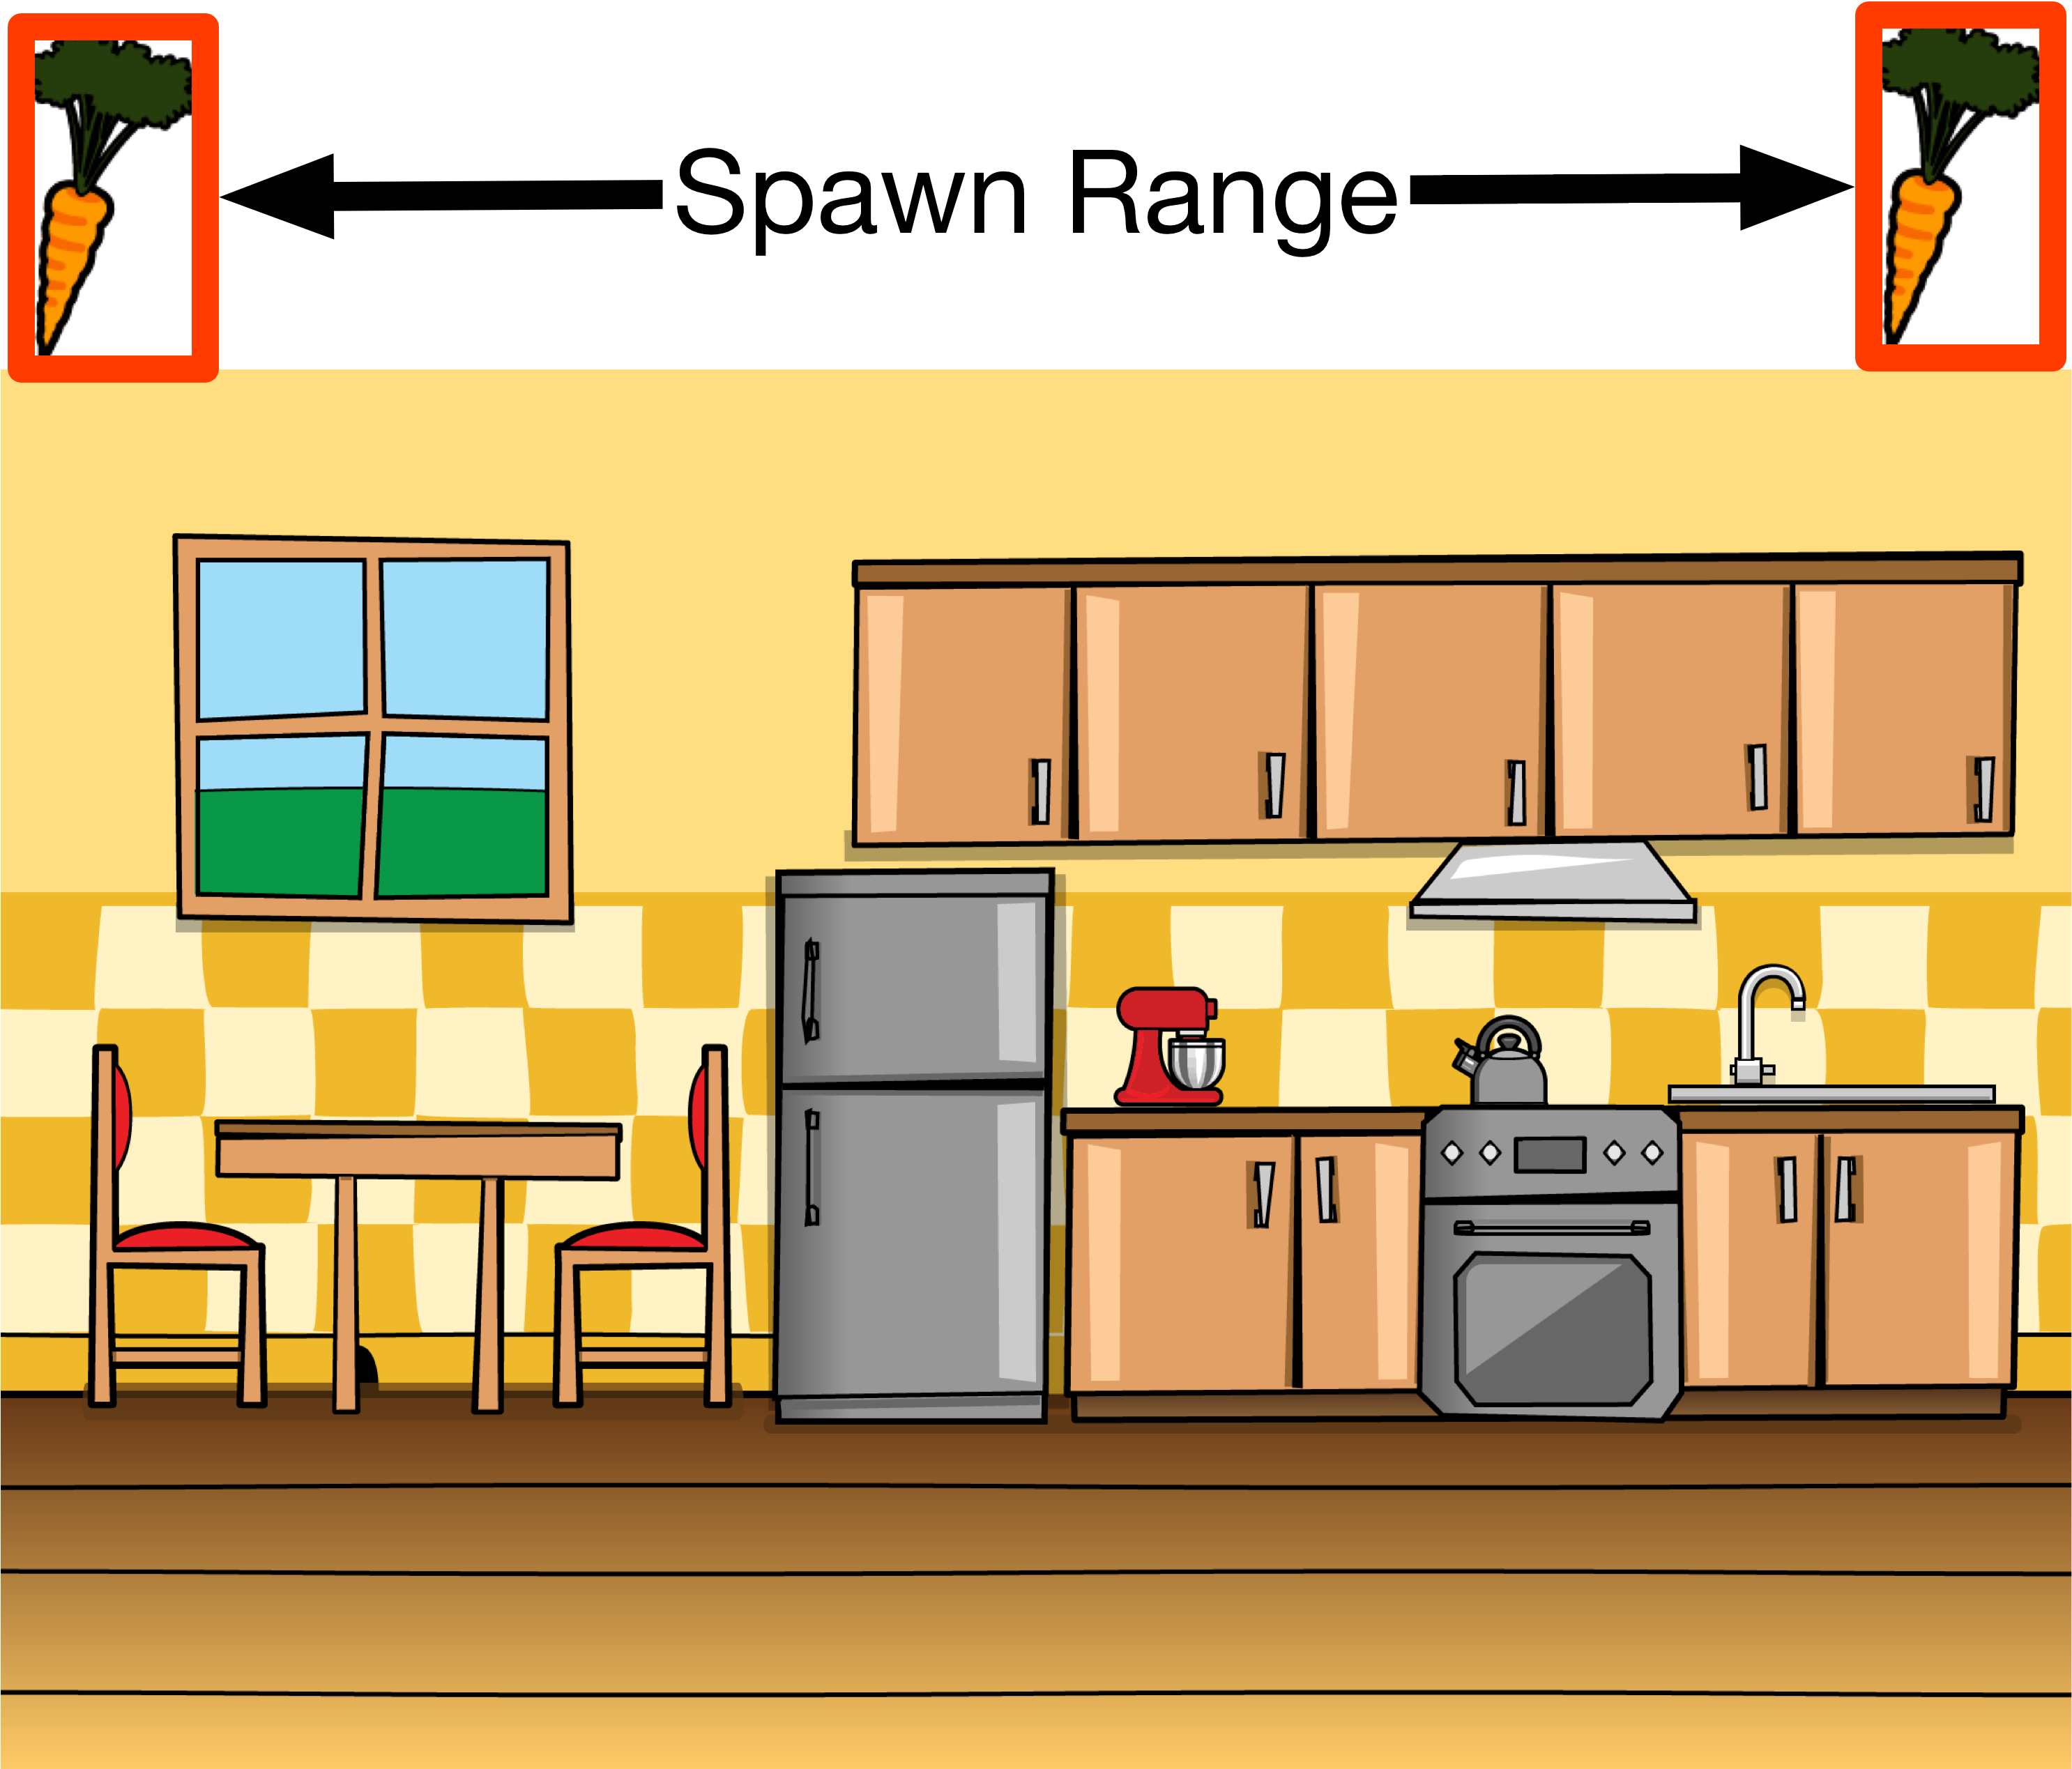
\includegraphics[width=170pt]{images/Chapter2/SpawnObjects.png}
\end{figure}

Our current version of the game spawns new objects twice a second at the top of
the screen and at a random X position. However, these objects don't move yet so
you won't be able to see them falling down. Let's implement the falling code to
complete the entire spawning functionality!

\section{Move falling objects}
The last step for this chapter will be making the objects we are spawning fall
to the ground. While building your very first \SB{} game you have learned to use
the \cocos{} action system to move nodes. The action system lets us describe changes over time, e.g. \textit{move 100 points to the right over 2
seconds}. Another option to move nodes that we haven't
discussed yet is using the \cocos{} \textit{update loop}\index{Update Loop}.

\subsection{Update Loop}
When we build games with \cocos{} the engine attempts to render 60 frames a
second and draws theses rendered frames to the screen of the device. 60 discrete
updates a second are so fast, that they appear as one continous movement to the
human eye. 

When we move objects between rendering frames, they will appear as
moving objects to the user. \cocos{} provides a method that is called directly before a frame is rendered, the \inlinecode{update} method.

The \inlinecode{update} method is defined as part of the
\inlinecode{CCSchedulerTarget}\index{Framework Classes|CCSchedulerTarget}
protocol. \inlinecode{CCNode} implements this protocol, that means any subclass
of \inlinecode{CCNode} can override the method. This is the signature of the
\inlinecode{update} method:
\begin{lstlisting}
func update(delta: CCTime)
\end{lstlisting}
We receive one parameter called \inlinecode{delta} from the \cocos{} framework.
The delta parameter contains the milliseconds since the \inlinecode{update}
method was called last. Most of the time this value will be \textit{0.0167}
milliseconds, which is 1/60 of a second. If the performance of our game drops
below 60 FPS this value will be higher, because the time between two rendered
frames will increase. If we want our objects to move at the same speed,
independent of the current framerate, we can use this delta parameter to
calculate how far we need to move nodes between two given frames.

Enough of the theory - let's implement our update method, that will help you
understand the details.

\subsection{Implementing the update method}
Here is what we want to do in the update method:

\begin{itemize}
  \item Iterate over all falling objects
  \item For each object check if it is within the screen boundaries
  \item If the object is outside of the screen, remove it
  \item If the object is inside of the screen boundary, let it fall to the
  bottom
\end{itemize}

\begin{leftbar}
Add the following \inlinecode{update} method to \inlinecode{MainScene}:
\begin{lstlisting}
  override func update(delta: CCTime) {
    // use classic for loop so that we can remove objects while iterating over the array
    for (var i = 0; i < fallingObjects.count; i++) {
      let fallingObject = fallingObjects[i]
      
      // check if falling object is below the screen boundary
      if (CGRectGetMaxY(fallingObject.boundingBox()) < CGRectGetMinY(boundingBox())) {
        // if object is below screen, remove it
        fallingObject.removeFromParent()
        fallingObjects.removeAtIndex(i)
      } else {
        // else, let the object fall with a constant speed
        fallingObject.position = ccp(
          fallingObject.position.x,
          fallingObject.position.y - CGFloat(fallingSpeed * delta)
        )
      }
    }
  }
\end{lstlisting}
\end{leftbar}

The interesting aspect of the code snippet above is how we check if the
falling object is out of bounds and how we move the falling object. Note that we
are using the \inlinecode{CGRectGetMaxY} and \inlinecode{CGRectGetMinY}
functions to determine the top and the bottom of the bounding boxes of the
falling object and the gameplay scene. The \inlinecode{CGRectGetMaxY} function
returns the largest Y value of the bounding box. Using these functions is preferred over accessing values
directly (e.g. \inlinecode{fallingObject.boundingBox.origin.y}) because they
also work for rectangles with negative sizes, e.g. a rectangle with a height of
\textit{-10} (which is technically possible in 2D math!).

If we detect that the top border of the falling object is below the bottom
border of the screen, we remove the falling object from the scene. We do that by
first calling \inlinecode{removeFromParent} on the node - which removes it from
the scene graph and makes it invisible. Then we additionally remove the node
from the \inlinecode{fallingObjects} array, so that the node gets destroyed and
the memory gets freed.

If the falling object is within the screen boundary we move it to the bottom
with the constant speed that we defined earlier multiplied by the value of
\inlinecode{delta}.

Now the falling mechanic is entirely implemented! In the next and last
section of this chapter you will learn how to add sound assets to the game.

\begin{details}[Update vs. Fixed Update] 
This chapter discusses the \inlinecode{update:} method of \cocos{} in detail.
\cocos{} provides a second similar method called
\inlinecode{fixedUpdate:}\index{Fixed Update}.
Unlike the \inlinecode{update:} method, the \inlinecode{fixedUpdate:} method is
\textbf{guaranteed} to be called at a specified interval (per default 1/60) and
is not dependent on the framerate the game is running at. The physics engine
integrated in \cocos{} uses the
\inlinecode{fixedUpdate:} method to perform all of its calculations. For you as
developer that means that you should implement code that changes physical
attributes in the \inlinecode{fixedUpdate:} method and \textbf{not} in the
\inlinecode{update:} method. Building games involving physics is not part of
this book. If you pursue a physics game on your own after finishing this book
you can read a nice blog post about the \inlinecode{fixedUpdate} method here:
\url{http://kirillmuzykov.com/update-vs-fixedupdate-in-cocos2d/}.
\end{details}

\section{Adding sound effects}
The goal of this chapter is for you to learn how to use assets with \SB{} and
\cocos{}. Obviously images are the most important assets in games, but sound
effects also play a big role in creating games that your players enjoy. In this
section you will learn how to add a sound effect that gets played whenever one
of the falling objects drops off the screen.

\SB{} is designed to take care of your entire asset management. This means that
you want to add all image files and all audio files to your \SB{} project.

All sound files need to be added to \SB{} projects in the \textit{Wave}
format. \SB{} will then generate compressed versions of that sound as you
publish the project. You can add the sound effect - just like any other asset -
by dragging it from Finder to the resource pane (in the bottom left) of \SB{}. For this project I have included a \filemention{drop.wav}
file in the \filemention{assets} folder that you downloaded and added to your
project earlier.

There are different ways to play sound effects added to your \SB{} project: you
can add a sound effect to a \SB{} timeline or you can play a sound effect
directly from code. We will first look at the timeline approach, later in the
book I will show you how to play sound effects in code.
Before we set up the sound effect I want to give you a basic introduction to the timeline feature
of \SB{} since it is one of the most powerful tools that \SB{} provides.

\subsection{\SB{}'s timeline feature}\index{\SB{} timeline}
The \SB{} timeline is a tool that allows developers to create animations and
sequences of sound effects without writing code. Every \ccbfile{} has one
\textit{Default Timeline} associated with it as soon as it is created. However,
a \ccbfile{} can, and often will, have multiple different timelines. Each
timeline is a sequence of sound effects, callbacks and most importantly
keyframes. Keyframes allow us to create animations by defining how sprites move
and change over time. We can change properties such as position, rotation,
color, etc. \SB{}'s animation tool is very similar to the famous Flash keyframe
editor. It is extremely useful in creating polished games and throughout later
parts of this book we will use the \SB{} timeline to create UI and game
animations.

Timelines can either be idle or playing. Timelines start playing in one of three
cases:
\begin{enumerate}
  \item \texit{Autoplay} is activated. That's the default setting for the
  \textit{Default Timeline}
  \item The timeline is triggered to play from code
  \item The timeline has been chained to another timeline
\end{enumerate}

We'll discuss each of these three cases as we use the timeline feature
throughout this book. 

You will get to know the value of \SB{}s timeline as we add more features to our
game.

\subsubsection{Adding the sound effect to a timeline}
For now let's take a look at how we can play sound effects using the timeline!

\begin{leftbar}
Start by creating a new timeline for the sound effect as shown in the following
screenshot: 

\begin{figure}[H]
    \centering
    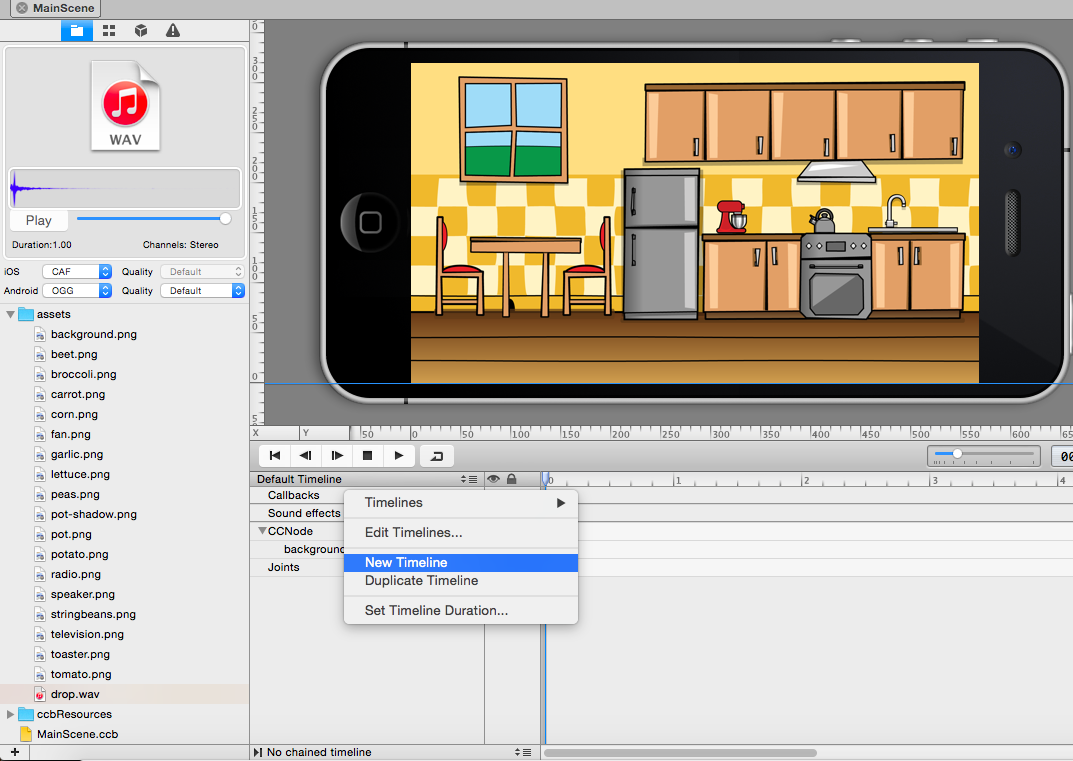
\includegraphics[width=0.9\linewidth]{images/Chapter2/new_timeline_audio.png}
    \caption{WAV files can be added by dragging them to the resource
    pane}\label{fig:audio_new_timeline}
\end{figure}
\end{leftbar}

Now we can add the audio file to this new timeline.

\begin{leftbar}
Take a look at the next image and follow the individual steps below it:
\begin{figure}[H]
    \centering
    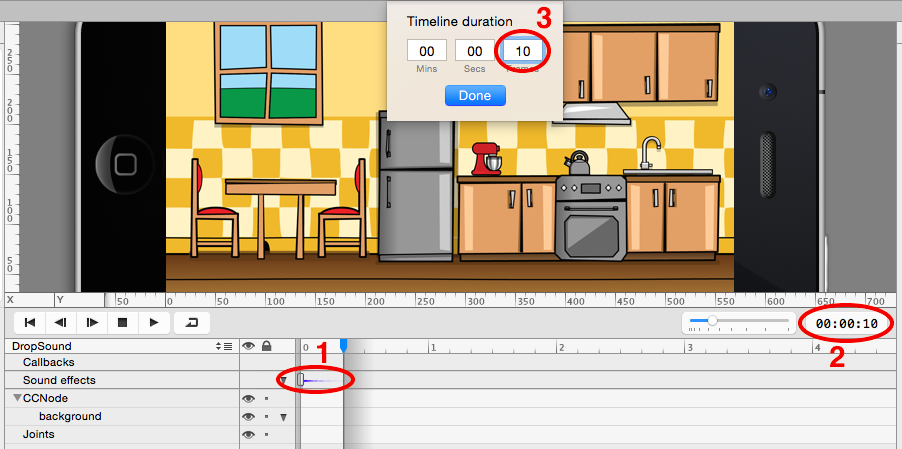
\includegraphics[width=0.9\linewidth]{images/Chapter2/audio_timeline.png}
\end{figure}
\begin{description}
\item[(1)] Drag the sound effect from the asset library in the left panel to the
\textit{Sound effects} row of \SB{}'s timeline (the second row from the top). When the sound
is added to the timeline it will be displayed in wave form.
\item[(2)] You should adjust the duration of the timeline to match the
duration of the sound effect. Click onto the time indicator to adjust the
timeline duration.
\item[(3)] In the popup that shows up next, change the timeline duration to 10
frames.
\end{description}
\end{leftbar}

Now the sound is ready to play! The last step is assigning a unique name to this
timeline which we can reference from code. You can rename a timeline by either
choosing \textit{Animation -> Edit Timelines\ldots} or selecting the dropdown
button next to the timeline name.

\begin{leftbar}
Rename the sound timeline to  \textit{DropSound}.
\begin{enumerate}
  \item Open the timeline editor dialog:
  \begin{figure}[H]
    \centering
    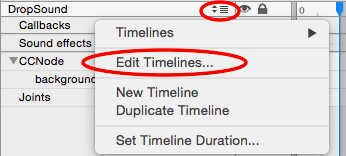
\includegraphics[width=200pt]{images/Chapter2/edit_timeline.png}
  \end{figure}
  \item Then rename the timeline by double-clicking onto the name:
  \begin{figure}[H]
    \centering
    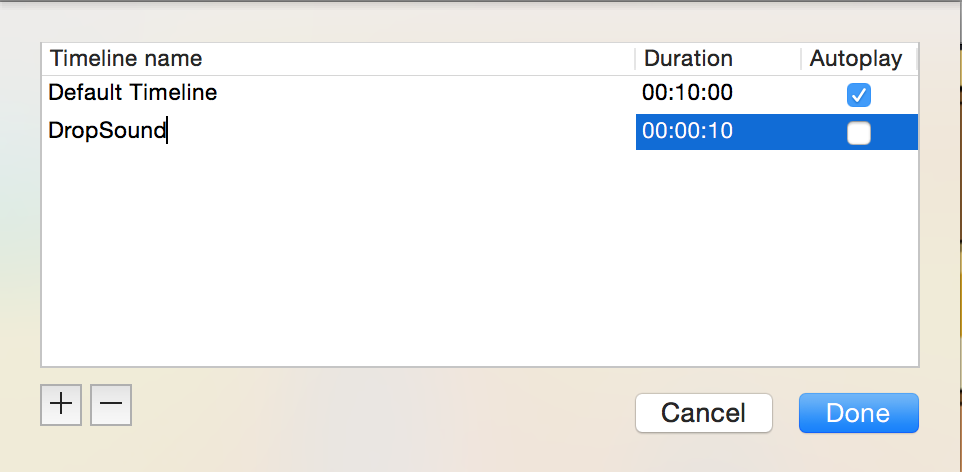
\includegraphics[width=200pt]{images/Chapter2/rename_timeline.png}
  \end{figure}
\end{enumerate}

\end{leftbar}

Now everything is set up and you can hit the publish button in \SB{}.

\begin{leftbar}
Publish the \SB{} project and switch to \xcode{}.
\end{leftbar}

\subsection{Triggering a Sound Effect}
Now we have set up the sound effect in \SB{} and published the project, all that
is left to do is to open the \xcode{} project and add code to play the sound
effect as soon as an object falls below the screen boundary.

We are going to implement this in \textit{SBBMainScene.m}. \cocos{} provides a
very simple API call to run a timeline animation from code. The following line
added to \inlinecode{SBBMainScene} will run the timeline animation and thus play the
sound we added to the project:
\begin{lstlisting}
animationManager.runAnimationsForSequenceNamed("DropSound")
\end{lstlisting}
The animation manager of the root node of a \ccbfile{} provides us access to the
different timelines and allows us to run and pause them and to react to their
completion - we will use these capabilities extensively throughout this book.

As mentioned earlier we want to play the sound effect when an object falls off
the screen. We already have code that checks for that condition in our
\inlinecode{update} method. All we need to do this to add the line that runs the
timeline. 

\begin{leftbar}
Extend the relevant part of the \inlinecode{update} method to look as
following:
\begin{lstlisting}
// check if falling object is below the screen boundary
if (CGRectGetMaxY(fallingObject.boundingBox()) < CGRectGetMinY(boundingBox())) {
	// if object is below screen, remove it
    fallingObject.removeFromParent()
    fallingObjects.removeAtIndex(i)
    // play sound effect
    animationManager.runAnimationsForSequenceNamed("DropSound")
} else {...}
\end{lstlisting}
\end{leftbar}

Now you can compile and test the project. Every time an object falls of the
screen you should hear the drop sound play!

\section{Wrapping up}
In this chapter you have learned how to work with an essential component of all
video games - image and audio assets. You have learned how to design scenes with
sprites in \SB{}, how to load and change sprite textures in code. You got to
know how \SB{} handles different asset resolutions for different screen and
device types and you have played your first sound effect. You have learned some
of the most important essentials of game development with \SB{} and \cocos{}.

The focus of the next chapter is \textit{User Interaction}. You will learn how
to incorporate user input into your game by implementing a drag and drop
mechanism!